% TEMPLATE for Usenix papers, specifically to meet requirements of
%  USENIX '05
% originally a template for producing IEEE-format articles using LaTeX.
%   written by Matthew Ward, CS Department, Worcester Polytechnic Institute.
% adapted by David Beazley for his excellent SWIG paper in Proceedings,
%   Tcl 96
% turned into a smartass generic template by De Clarke, with thanks to
%   both the above pioneers
% use at your own risk.  Complaints to /dev/null.
% make it two column with no page numbering, default is 10 point

% Munged by Fred Douglis <douglis@research.att.com> 10/97 to separate
% the .sty file from the LaTeX source template, so that people can
% more easily include the .sty file into an existing document.  Also
% changed to more closely follow the style guidelines as represented
% by the Word sample file. 

% Note that since 2010, USENIX does not require endnotes. If you want
% foot of page notes, don't include the endnotes package in the 
% usepackage command, below.

\documentclass[letterpaper,twocolumn,10pt]{article}
\usepackage[utf8]{inputenc}
\usepackage{t1enc}
\usepackage{usenix,epsfig,endnotes}
\usepackage{float}
\usepackage{graphicx}
\begin{document}

%don't want date printed
\date{}

%make title bold and 14 pt font (Latex default is non-bold, 16 pt)
\title{\Large Sistemas de Inteligencia Artificial \\
\Large \bf Algoritmos Genéticos \\
\Large Trabajo Práctico Especial N\textsuperscript{o} 5}

\author{
{\rm Juan Pablo Civile}
\and
{\rm Alvaro Crespo}
\and
{\rm Esteban Ordano}
}

\maketitle

% Use the following at camera-ready time to suppress page numbers.
% Comment it out when you first submit the paper for review.
\thispagestyle{empty}


\subsection*{Resumen}
Se implementó un motor de algoritmos genéticos con el objetivo de obtener los pesos de una
red neuronal multicapa que aprenda la siguiente función: $z(x, y) = c\sin(a x - b y)$.

\section{Descripción del Problema}

En el trabajo anterior, una arquitectura de una red neuronal encontrada óptima para el
problema en cuestión tenía 9 y 6 neuronas en sus capas ocultas, 2 entradas, y una capa de
salida de una neurona. Esto implica que los pesos entre las capas pueden representarse como
matrices de dimensiones 3x9, 10x6 y 7x1 respectivamente, lo que da un total de 94
valores. Estos 94 valores son los alelos de los cromosomas, los individuos de la
población.

Se utilizó el error cuadrático medio respecto de un conjunto de datos de prueba.
Por lo tanto, la función de \textit{fitness} se definió como el inverso multiplicativo
del error cuadrático medio, para que mayor \textit{fitness} se corresponda con una red
neuronal con menor error.

\section{Implementación}

\subsection{Método de Reemplazo}

Se implementaron los métodos de reemplazo presentados por la cátedra. El primero de ellos,
reemplaza toda la generación por nuevos individuos, provenientes de la recombinación
de individuos de la generación anterior. El segundo, un método con recambio
generacional que selecciona tanto individuos de la generación anterior como individuos
obtenidos a partir de la recombinación de individuos de la generación anterior. El tercero,
similar al segundo, genera nuevos individuos por recombinación y a través de un criterio de
selección, elige entre la generación anterior y estos nuevos individuos 
aquellos que formarán parte de la nueva generación.

\subsection{Operador Genético de Cruce}

Se implementaron los siguientes operadores genéticos de recombinación o cruce:

\begin{itemize}
    \item \textbf{Cruce de un punto}: Se elige un locus al azar y se intercambian los
    alelos de los dos individuos anteriores a partir de ese locus.
    \item \textbf{Cruce de dos puntos}: Se eligen dos locus al azar y se intercambian los
    alelos de los dos individuos anteriores entre estas dos posiciones.
    \item \textbf{Anular}: Se elige un locus al azar y se intercambian \textit{L} alelos
    a partir de ese locus. Se utilizó $L=10$ y $L=30$.
    \item \textbf{Cruce Uniforme Parametrizado}: Para cada locus, con una probabilidad
    determinada, se produce el cruce. Se utilizó una probabilidad de $0.6$.
\end{itemize}

\subsection{Operador Genético de Mutación}

Se implementaron dos ligeras variaciones del algoritmo de mutación. Ambas en sus versiones
con mutación simple y no uniforme.

\begin{itemize}
    \item \textbf{Mutación por individuo}: Se genera una mutación en el individuo con una
        probabilidad determinada, en un único locus seleccionado aleatoriamente.
    \item \textbf{Mutación simple}: Por cada locus, con una probabilidad
        determinada, se produce una mutación en ese alelo. Se utilizó una
        probabilidad de $0.01$.
\end{itemize}

Para las variaciones no uniformes, se utilizó $p_i = 0.995p_{i-1}$ y  $p_i = 0.999p_{i-1}$
(una variación de $0.5\%$ y $0.1\%$ por generación).

\subsection{Criterio de Selección}

Se implementaron los siguientes criterios de selección:

\begin{itemize}
    \item \textbf{Elitismo}: Se seleccionan los individuos de mayor \textit{fitness}.
    \item \textbf{Ranking}: La probabilidad de seleccionar un individuo es
        proporcional a su posición en una lista de los individuos ordenados por
        \textit{fitness}, de menor a mayor.
    \item \textbf{Ruleta}: La probabilidad de seleccionar un individuo es proporcional
        a su \textit{fitness}, y para cada individuo a seleccionar se utiliza un número
        aleatorio.
    \item \textbf{Estocástico}: La probabilidad de seleccionar un individuo es proporcional
        a su \textit{fitness}, pero se selecciona un solo número al azar.
    \item \textbf{Torneo}: Se seleccionan individuos en parejas al azar y se comparan sus
        valores de \textit{fitness}, y con una probabilidad determinada, se selecciona
        el de mayor o el de menor valor de \textit{fitness}. Se utilizó una probabilidad
        de $0.75\%$.
    \item \textbf{Boltzmann}: La probabilidad de seleccionar un individuo es función
        de su \textit{fitness} y de la cantidad de generaciones. Se utilizaron temperaturas
        $T=g$ y $T=0.5g$, donde $g$ es la cantidad de generaciones desde la primera.
    \item \textbf{Mixto}: Seleccionar los individuos según distintos criterios. Se
        utilizaron las variantes:
    \begin{itemize}
        \item \textbf{Mix Estocástico y Elitismo}: Se selecciona un $30\%$ de individuos
            según el criterio de elitismo, y el procentaje restante de acuerdo al criterio
            estocástico. También se utilizó $70\%$ según el criterio estocástico y $30\%$
            según el criterio de elitismo.
        \item \textbf{Mix Ruleta y Elitismo}: De manera similar al punto anterior, pero
            utilizando el criterio de ruleta en vez del estocástico.
    \end{itemize}
\end{itemize}

\subsection{Criterio de Corte}

Se implementaron los siguientes criterios de corte:

\begin{itemize}
    \item \textbf{Cantidad de Generaciones}: El algoritmo se ejecuta hasta llegar a un
    límite máximo de generaciones creadas.
    \item \textbf{Estructura similar}: El algoritmo se ejecuta hasta que se detecta que
    generaciones sucesivas están compuestas de individuos muy similares. Se comparan las
    diferencias absolutas entre los alelos de todos los individuos. Una variante de este
    criterio es seleccionar un muestreo al azar de individuos de ambas generaciones.
    \item \textbf{Contenido similar}: El mejor \textit{fitness} de la población no varía
    con el tiempo.
    \item \textbf{\textit{Fitness} buscado}: El algoritmo se ejecuta hasta que el mejor
    \textit{fitness} de una generación supera una cota determinada.
    \item \textbf{Criterio mixto}: El algoritmo corta cuando se dá una de dos condiciones:
        el mejor \textit{fitness} supera un valor buscado o la cantidad de
        generaciones supera una cantidad límite.
\end{itemize}

El criterio utilizado en todas las pruebas realizadas fue un criterio mixto, donde el 
algoritmo detenía su ejecución después de $200$ generaciones o al alcanzar un
\textit{fitness} de $1000$.

\subsection{Explosión combinatoria}

La numerosa cantidad de parámetros variables del motor de algoritmos genéticos
presenta la dificultad de que conseguir una configuración óptima sea muy complejo.

En particular, para los métodos de reemplazo 2 y 3, se deben elegir dos criterios de
selección (que pueden ser distintos), con lo cual teniendo 10 criterios de selección, son
100 distintas combinaciones. Otro parámetro que entra en juego aquí es el coeficiente
de reemplazo generacional.

En todo método de reemplazo, también se debe elegir entre 5 operadores genéticos de
recombinación, 4 operadores genéticos de mutación.

Todas estas distintas opciones se traducen en una cantidad de ejecuciones del
algoritmo genético en el orden de $10^5$, si el objetivo es comparar todas las
posibles configuraciones del motor. Dado que esta cantidad de ejecuciones escapa al poder
de cómputo disponible se decidió hacer un analisis reducido.

Se estudió:
\begin{itemize}
  \item \textbf{Cantidad de épocas de \textit{backpropagation}}: Se seleccionó una
    cantidad de épocas de backpropagation en una solución de compromiso entre resultados
    obtenidos y velocidad de ejecución.
  \item \textbf{Cantidad de individuos por generación}: Se buscó una cantidad de
    individuos que genere resultados aceptables sin requerir mucho poder de procesamiento.
  \item \textbf{Criterio de selección}: Se buscó, utilizando el método de reemplazo 1, sin
    mutaciones, y con cruce de un punto, cuál es el método de selección que dió
    mejores resultados para valores de $N = 80$.
  \item \textbf{Operadores genéticos de Cruce}: Utilizando el método de
    reemplazo 1 y el criterio de selección mixto (estocástico y 30\% elitismo), se buscó
    el mejor de los operadores genéticos de cruce para $N = 80$.
  \item \textbf{Criterio de selección para reemplazo}: Se buscó el mejor método de
    selección para ejecutar el reemplazo generacional en el método de reemplazo 2.
    Se utilizó un valor de $N = 80$ y se probó con un coeficiente de reemplazo
    generacional de 60\%.
  \item \textbf{Comparación entre métodos de reemplazo}: Se compararon los métodos de
    reemplazo 2 y 3 con los mejores algoritmos de selección encontrados.
\end{itemize}

\section{Resultados}
\label{sec:res}

\subsection{Backpropagation}

Se ejecutó el algoritmo genético con una cantidad de ejecuciones del algoritmo de
\textit{backpropagation} muy chica (entrenando la red unas 2000 veces a lo largo de
distintas generaciones). Los resultados son comparables con aquellos obtenenidos 
de una red neuronal con valores
seleccionados aleatoriamente, como se muestra en el anexo en \ref{img:no_backpropagation}.

Se utilizó una probabilidad de $0.05$ de ejecutar el algoritmo de \textit{backpropagation}
con un conjunto de entrenamiento de $400$ elementos y $40$ épocas del algoritmo. Estos
valores no son óptimos, si no que fueron elegidos para poder comparar los distintos
parámetros de configuración utilizando poco poder de procesamiento.

\subsection{Número de individuos por Generación}

En la figura \ref{img:selection_n} del anexo, se comparan los promedios de ejecución con
distintos métodos de selección para distintos valores de $N$. Se utilizó $N=80$ en todas
las sucesivas pruebas.

\subsection{Operador genético de Cruce}

La tabla \ref{fig:crossover} muestra los valores obtenidos de ejecuciones
con distintos operadores de cruce y los resultados obtenidos. A partir de estos resultados
se decidio fijar el operador de Cruce a Anular con $L = 10$.

\begin{table}[H]

\begin{center}
\begin{tabular}{l | r | r}
Criterio & Mejor & Promedio \\
\hline
Uniform Crossover 0.6 & $195.928$ & $178.646$ \\
Single Crossover & $389.887$ & $356.701$ \\
Double Crossover & $423.335$ & $408.75$ \\
Anular, L = 30 & $196.316$ & $280.827$ \\
Anular, L = 10 & $524.731$ & $524.731$ \\
\end{tabular}
\end{center}

\caption{Fitness obtenida para los distintos operadores de Crossover}
\label{fig:crossover}

\end{table}

\subsection{Selección de individuos}

Para el método de reemplazo 1, la tabla \ref{fig:seleccion} muestra, luego de 200
generaciones, los valores de fitness obtenidos. El operador genético de cruce utilizado
fue anular con $L=10$. En el anexo (figuras \ref{img:elite}, \ref{img:mix},
\ref{img:ranking}, \ref{img:tournament}, \ref{img:ruleta}) se muestra
la evolución a lo largo de distintas generaciones de algunos de estos algoritmos.
A partir de esto, se fijo el metodo de seleccion de cruce como Mix Roulette + 70\% Elite.

\begin{table}[H]

\begin{center}
\begin{tabular}{l | r | r}
Método & Mejor & Promedio \\
\hline
Tournament $0.75$ & $449.918$ & $447.498$ \\
Roulette & $380.219$ & $149.6$ \\
Rank & $232.019$ & $232.019$ \\
Elite & $277.545$ & $264.440$ \\
Boltzmann T = generations & $320.483$ & $306.531$ \\
Boltzmann T = 0.5 * generations & $170.122$ & $161.708$ \\
Mix Stochastic + 70\% Elite & $267.148$ & $252.895$ \\
Mix Roulette + 70\% Elite & $505.591$ & $446.057$ \\
Mix Roulette + 30\% Elite & $447.594$ & $399.834$ \\
Mix Stochastic + 30\% Elite & $515.609$ & $506.539$ \\
\end{tabular}
\end{center}

\caption{Valores de fitness para distintos métodos de selección}
\label{fig:seleccion}

\end{table}

\subsection{Método de Reemplazo 2}

Se buscó un valor para G, usando Mix Stochastic + Elite 30\% y luego elitismo:
\begin{table}[H]

\begin{center}
\begin{tabular}{l | r | r}
G & Mejor & Promedio \\
\hline
$0.6$ & $524.731$ & $524.731$ \\
$0.75$ & $364.749$ & $353.851$ \\
$0.9$ & $284.096$ & $273.342$ \\
\end{tabular}
\end{center}

\caption{Fitness obtenido para distintos valores de G}
\label{fig:g-reemplazo2}

\end{table}

Selección de los individuos de la nueva generación:
\begin{table}[H]

\begin{center}
\begin{tabular}{l | r | r}
Criterio & Mejor & Promedio \\
\hline
Tournament 0.75 & $345.249$ & $289.807$ \\
Roulette & $377.249$ & $361.807$ \\
Rank & $508.293$ & $495.604$ \\
Elite & $375.369$ & $365.45$ \\
Boltzmann T = generations & $284.096$ & $273.342$ \\
Mix Stochastic + 30\% Elite & $364.749$ & $353.851$ \\
Mix Roulette + 30\% Elite & $450.569$ & $446.164$ \\
\end{tabular}
\end{center}

\caption{Fitness para los distintos métodos de selección}
\label{fig:seleccion-reemplazo2}

\end{table}

\subsection{Método de Reemplazo 3}

La \ref{fig:reemplazo3} muestra una comparación entre los promedios de los mejores
individuos y los promedios de los valores de \textit{fitness} obtenidos utilizando
estos dos métodos, con distintos algoritmos de selección. Se muestra una evolución
del mejor individuo en cada generación para las mejores ejecuciones de los tres
métodos de reemplazo en la figura \ref{img:comparacion_reemplazo}.

\begin{table}[H]

\begin{center}
\begin{tabular}{l | r | r}
Método & Mejor & Promedio \\
\hline
Reemplazo 2 & $508.293$ & $495.604$ \\
Reemplazo 3 & $386.398$ & $342.212$ \\
\end{tabular}
\end{center}

\label{fig:reemplazo3}
\caption{Promedio de los mejores valores y el promedio generacional
luego de 200 generaciones para distintas ejecuciones del algoritmo}

\end{table}

\section{Conclusión}

En los resultados observados utilizando backpropagation como operador en el 
algoritmo genético (sección \ref{sec:res}), se encontró que buenos
parámetros para el motor son: utilizar el método de reemplazo 2, con
el método de selección para cruce \"mix estocástico + 30\% elite\",
método de selección para reemplazo generacional \"ranking\", operador
de cruce \"anular, L=10\", y un coeficiente de reemplazo generacional $G=0.6$.

En el trabajo práctico anterior, utilizando meramente el algoritmo de
\textit{backpropagation} se obtuvo una red con un error cuadrático medio de $0.00025$. 
La mejor red obtenida con algoritmos genéticos tuvo un valor de \textit{fitness} de
$764.166$, es decir, un error cuadrático medio de $0.00130$.

El uso de \textit{backpropagation} mejora sustancialmente los individuos de la
población a través de las generaciones. Si se considera a \textit{backpropagation} un
operador genético, se puede decir que es conciente de cómo funciona una red neuronal,
mientras que los algoritmos de crossover implementados no consideran a la estructura
si no como un vector de números.

De lo anterior se concluye que mejores resultados se obtendrían si el operador de
cruce estuviese diseñado especificamente para el problema de redes neuronales, con
backpropagation en todos los individuos. También sería interesante analizar cómo
este operador de cruce podría considerar redes neuronales de distintas estructuras,
incluso eliminando conexiones entre distintas neuronas o agregando capas.

Por último, el poder de procesamiento requerido para ejecutar el algoritmo genético
con estas condiciones es uno o dos órdenes de magnitud superior al algoritmo de
\textit{backpropagation}, pero esto es evidente por estar realizando operaciones con
$N$ redes neuronales.

\newpage

\section{Anexo}

\begin{figure}[h]

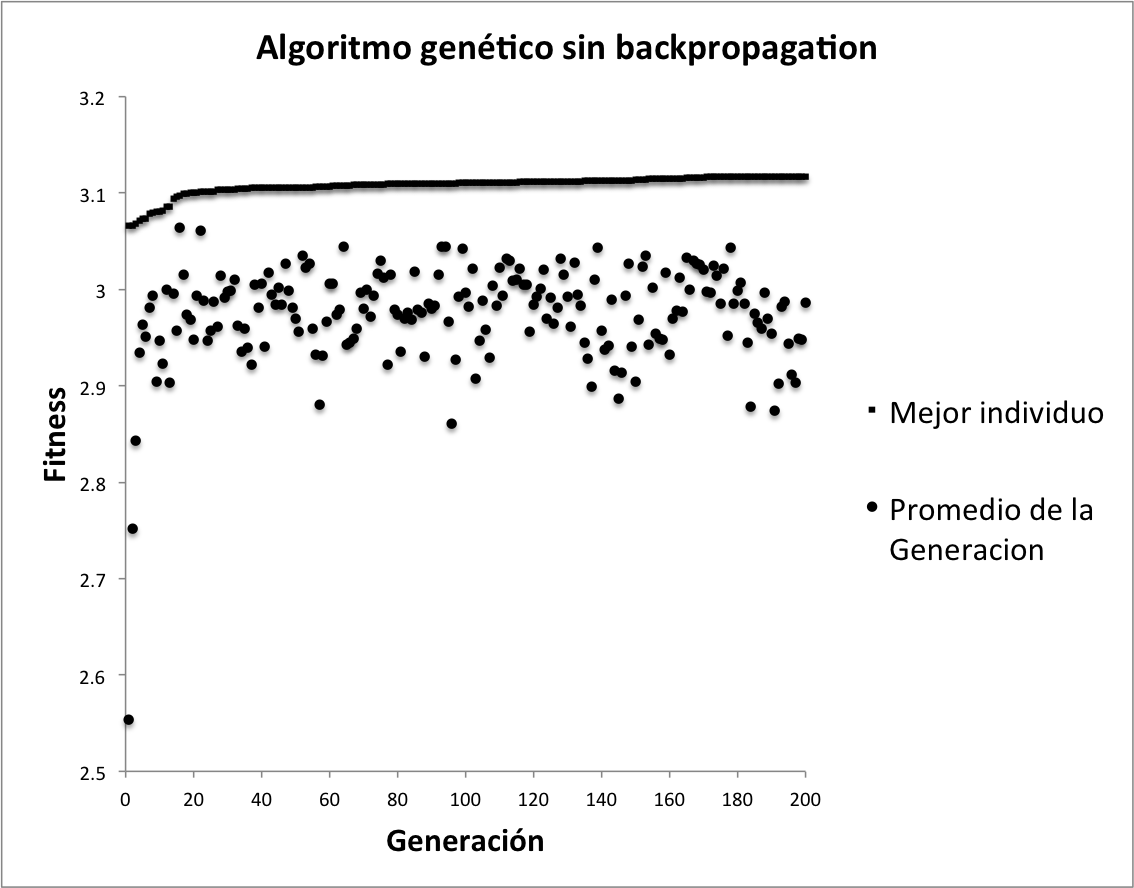
\includegraphics[width=0.5\textwidth]{No_Backpropagation.png}

\caption{}
\label{img:no_backpropagation}

\end{figure}

\begin{figure}[h]

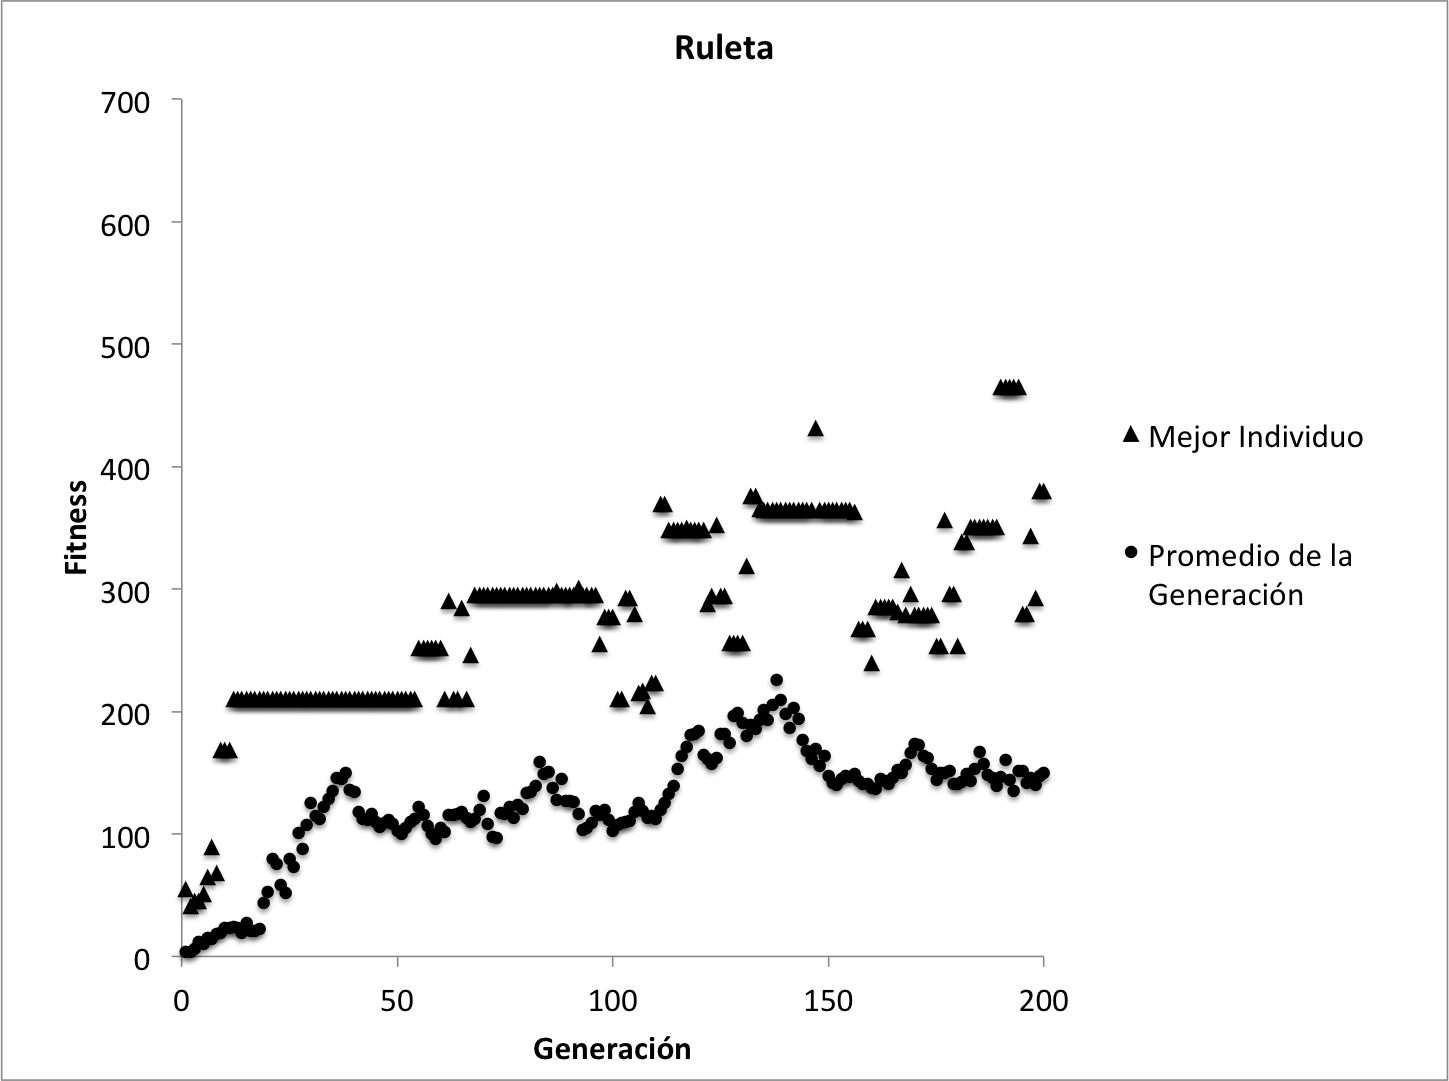
\includegraphics[width=0.5\textwidth]{Ruleta.png}

\caption{}
\label{img:ruleta}

\end{figure}

\begin{figure}[h]

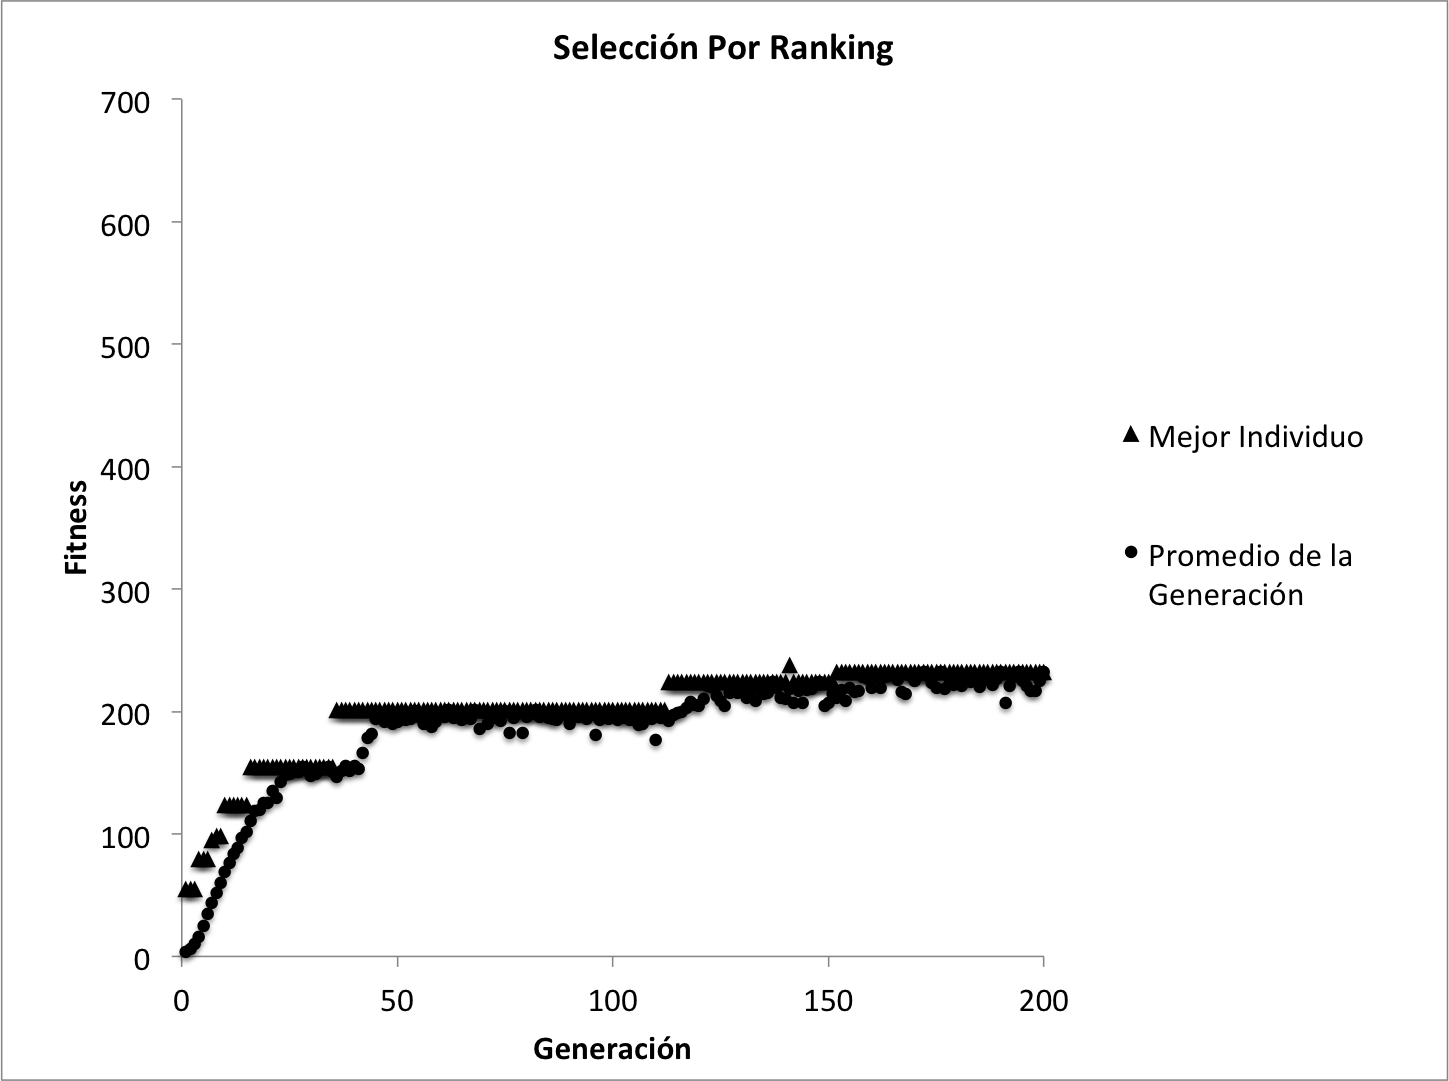
\includegraphics[width=0.5\textwidth]{Ranking.png}

\caption{}
\label{img:ranking}

\end{figure}

\begin{figure}[h]

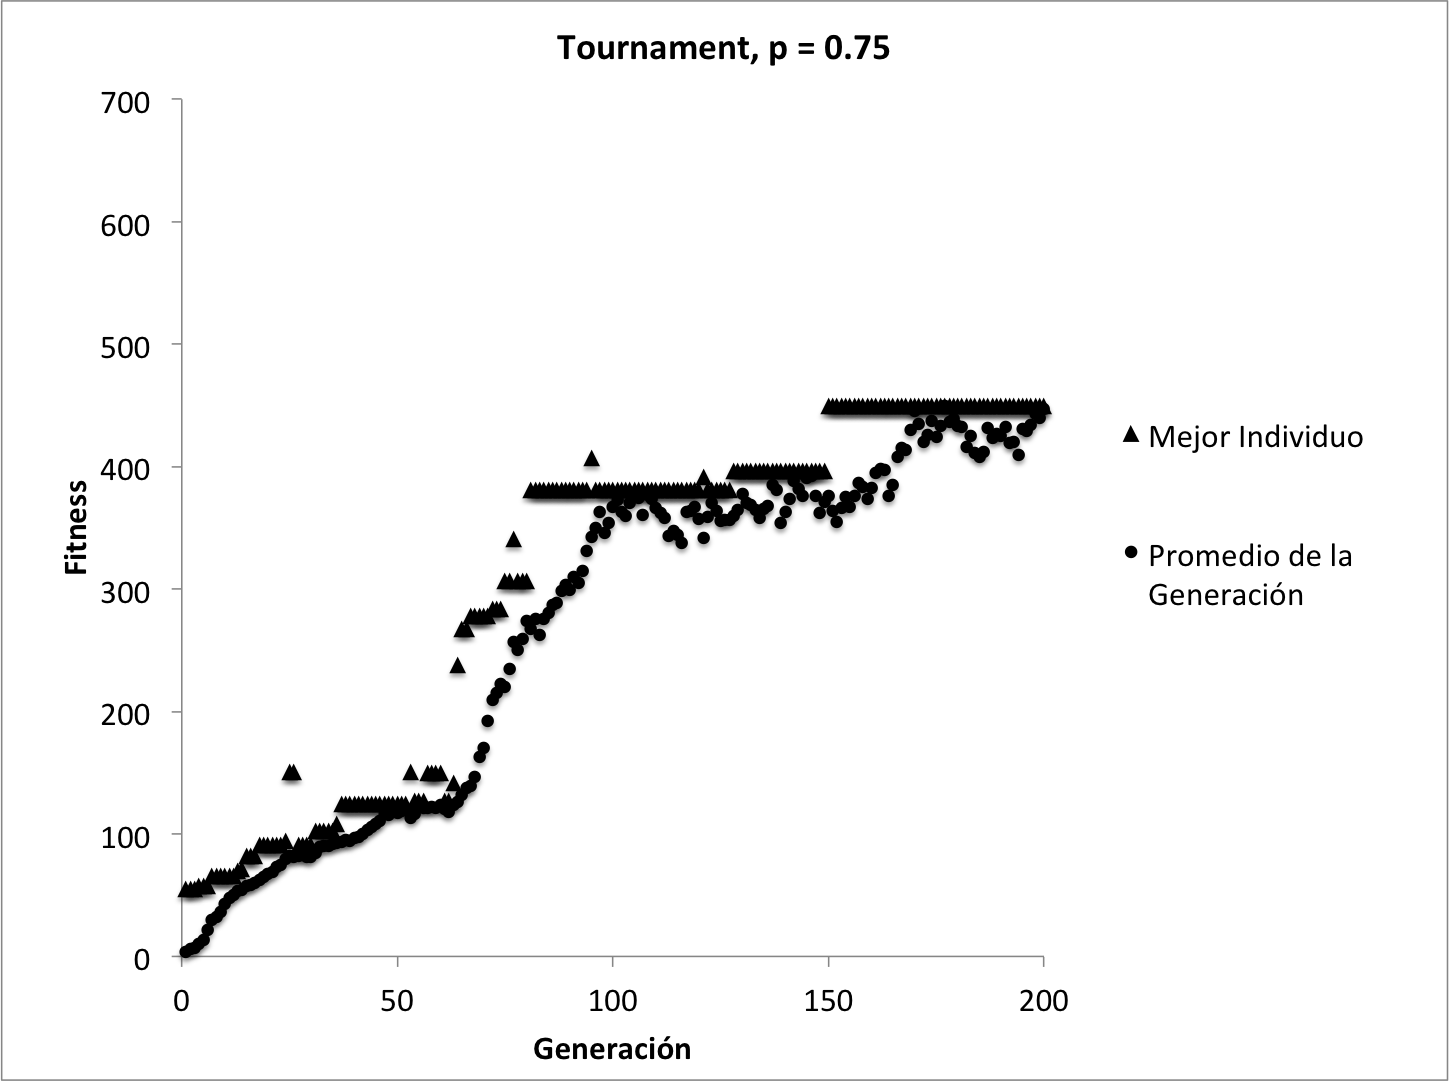
\includegraphics[width=0.5\textwidth]{Tournament.png}

\caption{}
\label{img:tournament}

\end{figure}

\begin{figure}[h]

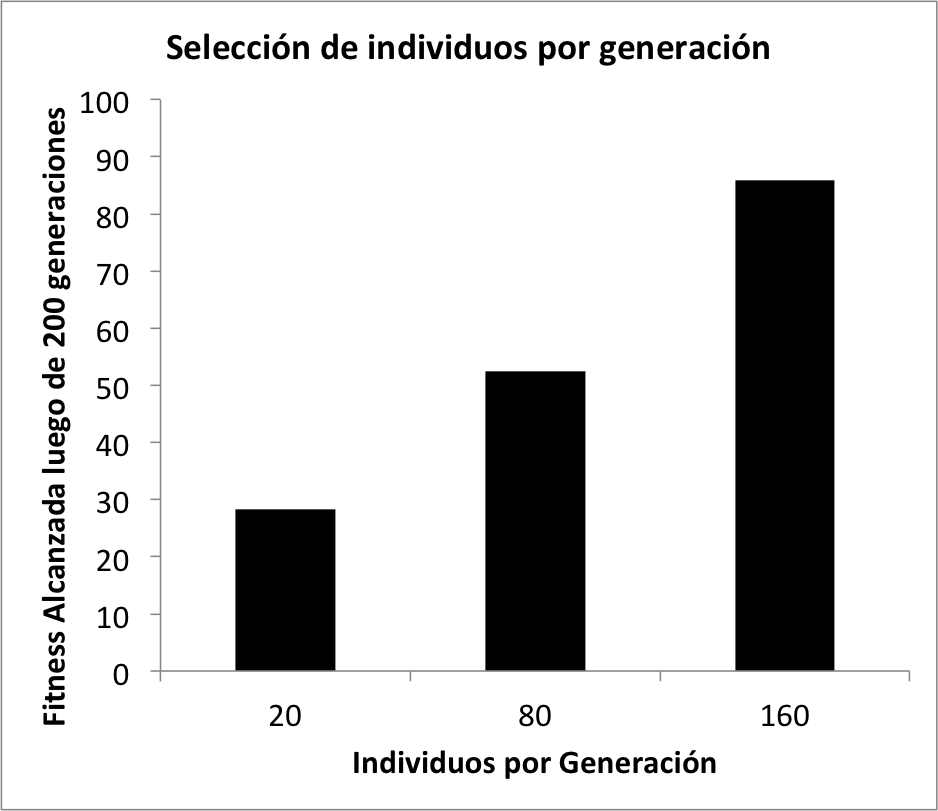
\includegraphics[width=0.5\textwidth]{Selection_N.png}

\caption{}
\label{img:selection_n}

\end{figure}

\begin{figure}[h]

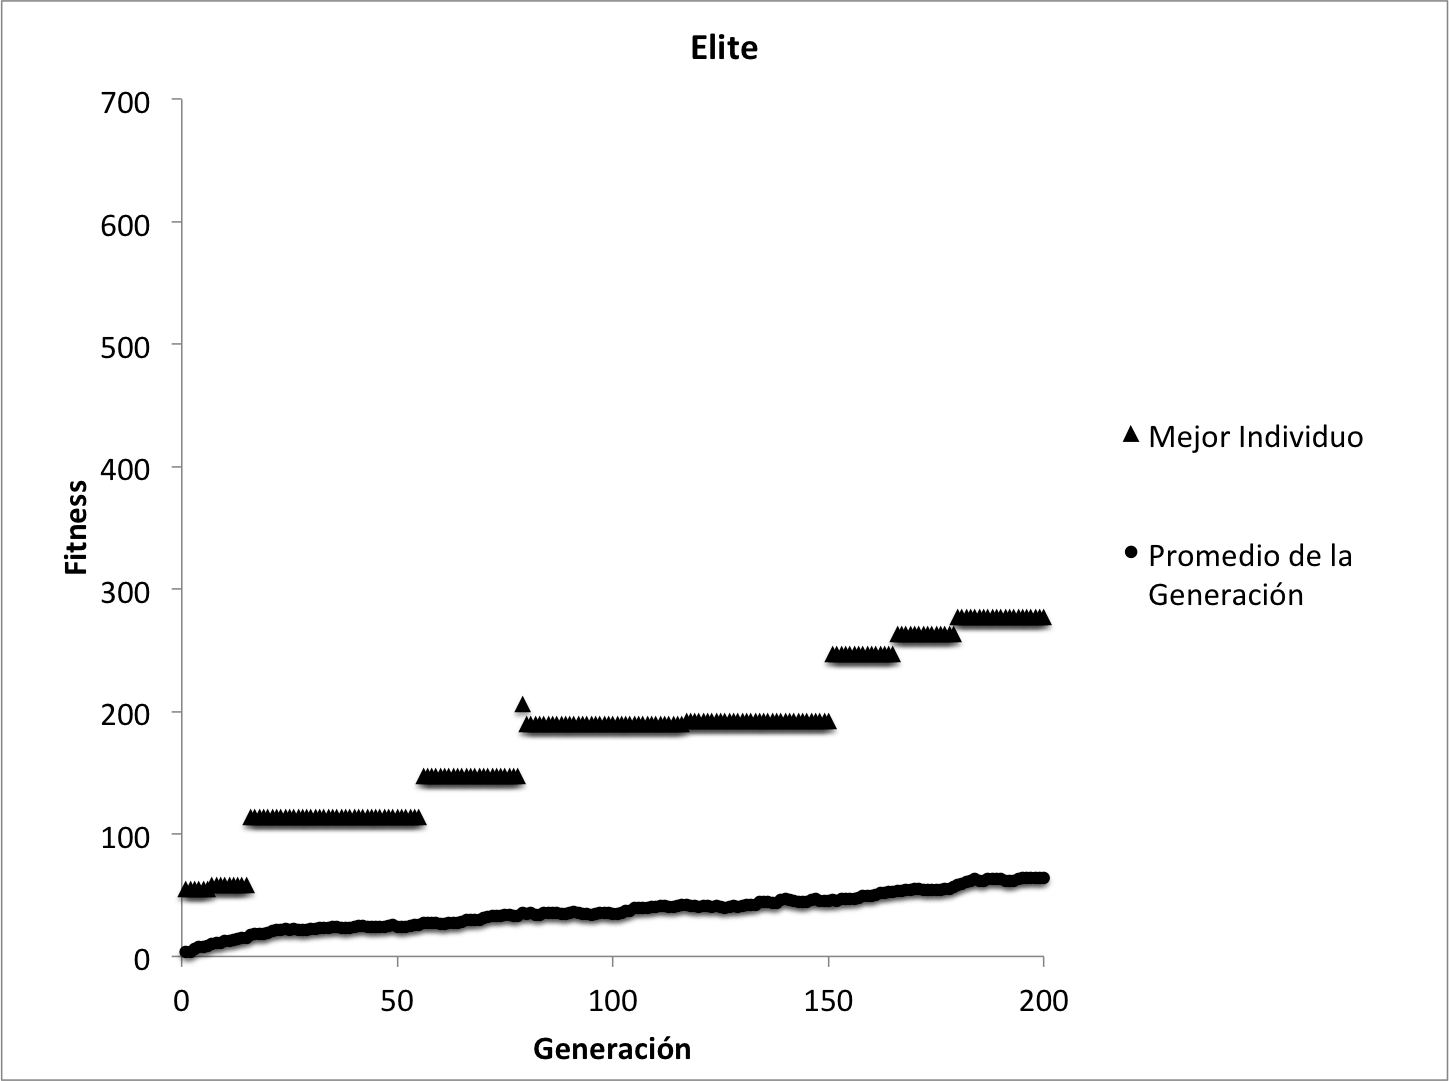
\includegraphics[width=0.5\textwidth]{Elite.png}

\caption{}
\label{img:elite}

\end{figure}

\begin{figure}[h]

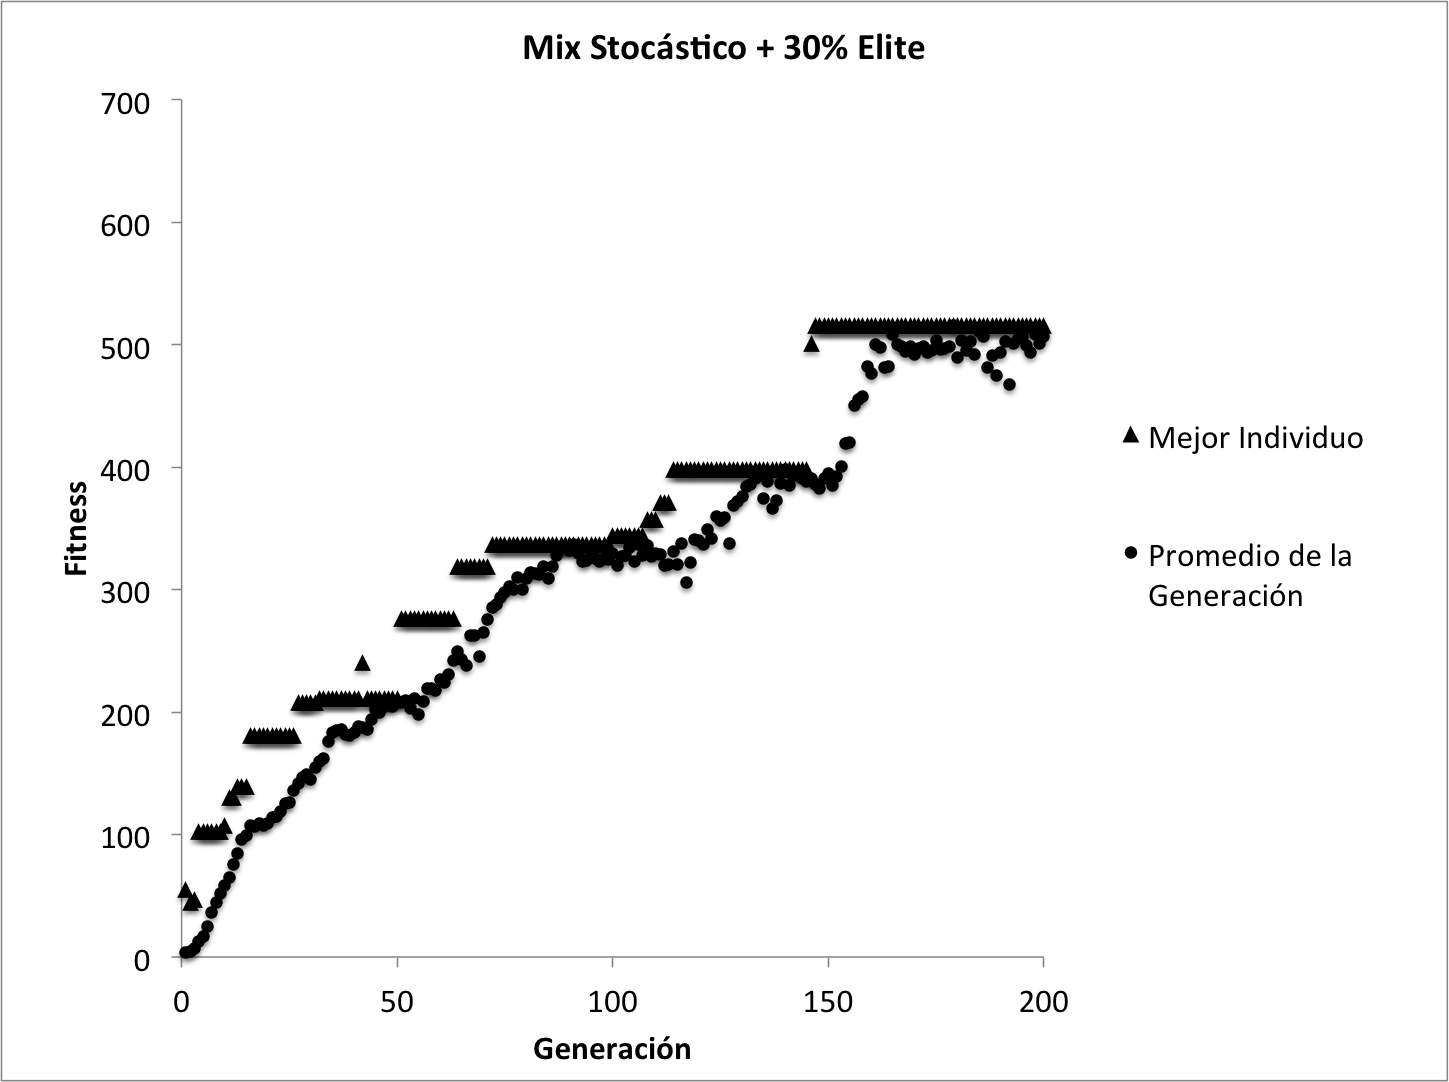
\includegraphics[width=0.5\textwidth]{Mix.png}

\caption{}
\label{img:mix}

\end{figure}

\begin{figure}[h]

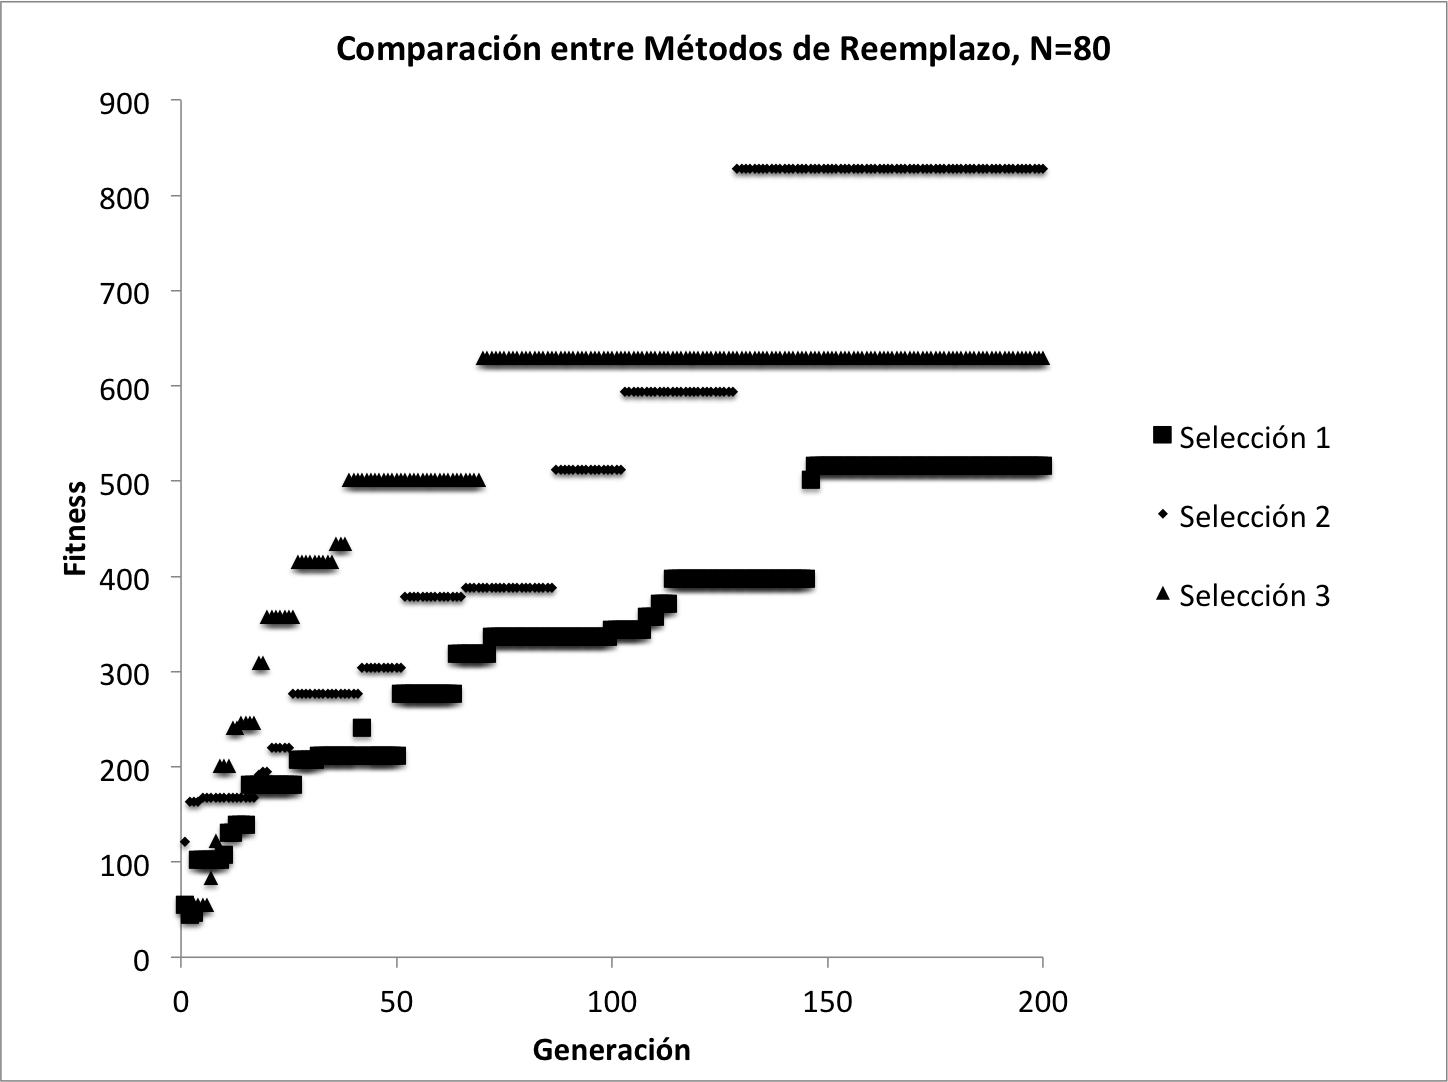
\includegraphics[width=0.5\textwidth]{Comparacion_Reemplazo.png}

\caption{}
\label{img:comparacion_reemplazo}

\end{figure}

\end{document}
